\documentclass[tikz,border=1.35mm]{standalone}
\usetikzlibrary{arrows.meta}

\definecolor{externalface}{HTML}{8FB9E8}
\definecolor{centroidgreen}{HTML}{0E8814}

% Exploded view of cell-based isotropic refinement for a hexahedron.
% Each original face becomes the base of a pyramid whose apex is a duplicated
% copy of the volume centroid.
\begin{document}
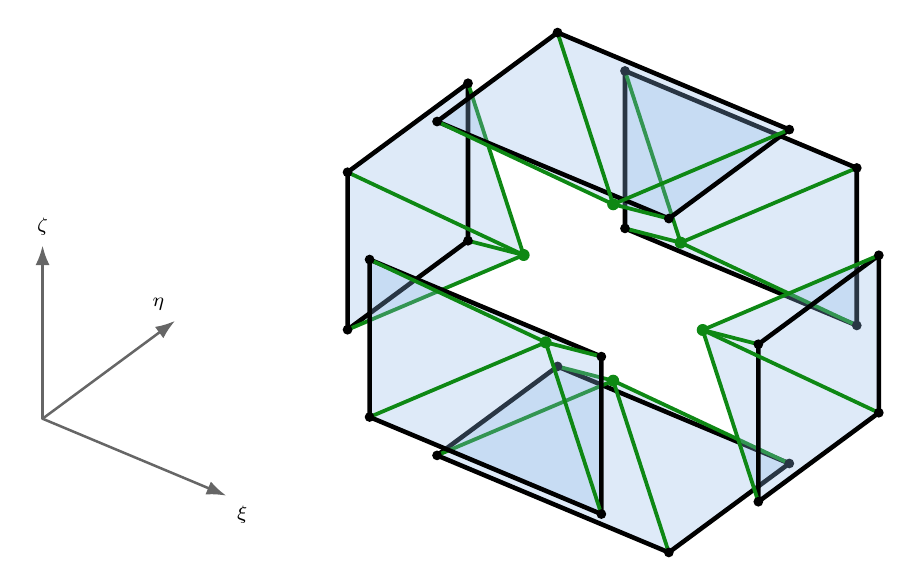
\begin{tikzpicture}[
  x={(20.3mm,-8.5mm)},
  y={(15.3mm,11.3mm)},
  z={(0mm,20mm)},
  line join=round,
  line cap=round,
  outer/.style={draw=black,line width=0.58mm},
  cellface/.style={fill=externalface,fill opacity=0.16,draw=none},
  centroidedge/.style={draw=centroidgreen,line width=0.48mm},
  axis/.style={draw=black!60,line width=0.32mm,-{Latex[length=2.5mm,width=1.8mm]}}
]
  \newcommand{\drawpyramid}[5]{%
    \path[cellface] (#1) -- (#2) -- (#3) -- (#4) -- cycle;
    \path[cellface] (#1) -- (#2) -- (#5) -- cycle;
    \path[cellface] (#2) -- (#3) -- (#5) -- cycle;
    \path[cellface] (#3) -- (#4) -- (#5) -- cycle;
    \path[cellface] (#4) -- (#1) -- (#5) -- cycle;
    \draw[outer] (#1) -- (#2) -- (#3) -- (#4) -- cycle;
    \foreach \p in {#1,#2,#3,#4} {
      \draw[centroidedge] (#5) -- (\p);
    }
    \foreach \p in {#1,#2,#3,#4} {
      \fill[black] (\p) circle[radius=0.62mm];
    }
    \fill[centroidgreen] (#5) circle[radius=0.76mm];
  }

  % Compact orientation axes, tucked away from the exploded cells.
  \coordinate (Oaxis) at (-1.85,-0.82,-0.65);
  \draw[axis] (Oaxis) -- (-0.70,-0.82,-0.65) node[below right,font=\scriptsize] {$\xi$};
  \draw[axis] (Oaxis) -- (-1.85,0.28,-0.65) node[above left,font=\scriptsize] {$\eta$};
  \draw[axis] (Oaxis) -- (-1.85,-0.82,0.45) node[above,font=\scriptsize] {$\zeta$};

  % Bottom and top pyramids.
  \coordinate (bA) at (0,0,-0.56);
  \coordinate (bB) at (1.45,0,-0.56);
  \coordinate (bC) at (1.45,1,-0.56);
  \coordinate (bD) at (0,1,-0.56);
  \coordinate (bO) at (0.725,0.5,-0.06);
  \coordinate (tE) at (0,0,1.56);
  \coordinate (tF) at (1.45,0,1.56);
  \coordinate (tG) at (1.45,1,1.56);
  \coordinate (tH) at (0,1,1.56);
  \coordinate (tO) at (0.725,0.5,1.06);

  % Front/back and left/right pyramids.
  \coordinate (fA) at (0,-0.56,0);
  \coordinate (fB) at (1.45,-0.56,0);
  \coordinate (fF) at (1.45,-0.56,1);
  \coordinate (fE) at (0,-0.56,1);
  \coordinate (fO) at (0.725,-0.06,0.5);
  \coordinate (kD) at (0,1.56,0);
  \coordinate (kC) at (1.45,1.56,0);
  \coordinate (kG) at (1.45,1.56,1);
  \coordinate (kH) at (0,1.56,1);
  \coordinate (kO) at (0.725,1.06,0.5);
  \coordinate (lD) at (-0.56,1,0);
  \coordinate (lA) at (-0.56,0,0);
  \coordinate (lE) at (-0.56,0,1);
  \coordinate (lH) at (-0.56,1,1);
  \coordinate (lO) at (0.165,0.5,0.5);
  \coordinate (rB) at (2.01,0,0);
  \coordinate (rC) at (2.01,1,0);
  \coordinate (rG) at (2.01,1,1);
  \coordinate (rF) at (2.01,0,1);
  \coordinate (rO) at (1.285,0.5,0.5);

  % Draw the six face pyramids. Back and bottom are drawn first.
  \drawpyramid{bA}{bB}{bC}{bD}{bO}
  \drawpyramid{kD}{kC}{kG}{kH}{kO}
  \drawpyramid{lD}{lA}{lE}{lH}{lO}
  \drawpyramid{rB}{rC}{rG}{rF}{rO}
  \drawpyramid{fA}{fB}{fF}{fE}{fO}
  \drawpyramid{tE}{tF}{tG}{tH}{tO}
\end{tikzpicture}
\end{document}
